\section{Model Introduction}
The Spacecraft Model's intention is to create model based estimates for key metrics associated with the design of an asteroid mining spacecraft. 
These metrics include, but are not limited to:
\begin{itemize}
    \item Dry mass
    \item Spacecraft cost
    \item Energy use
    \item Stay time
    \item Propellant usage
\end{itemize} 
These outputs are tightly correlated and cannot be solved for in isolation. This document will elaborate on how the Spacecraft Dry Mass is determined. 
The other output parameters, as mentioned, are closely correlated to the dry mass and their calculations can be easily inferred.
\newline
\autoref{fig-model-structure} describes how the dry mass model was broken down. This document will follow a similar structure for consistency. 

\begin{figure}[htb]
    \centering
    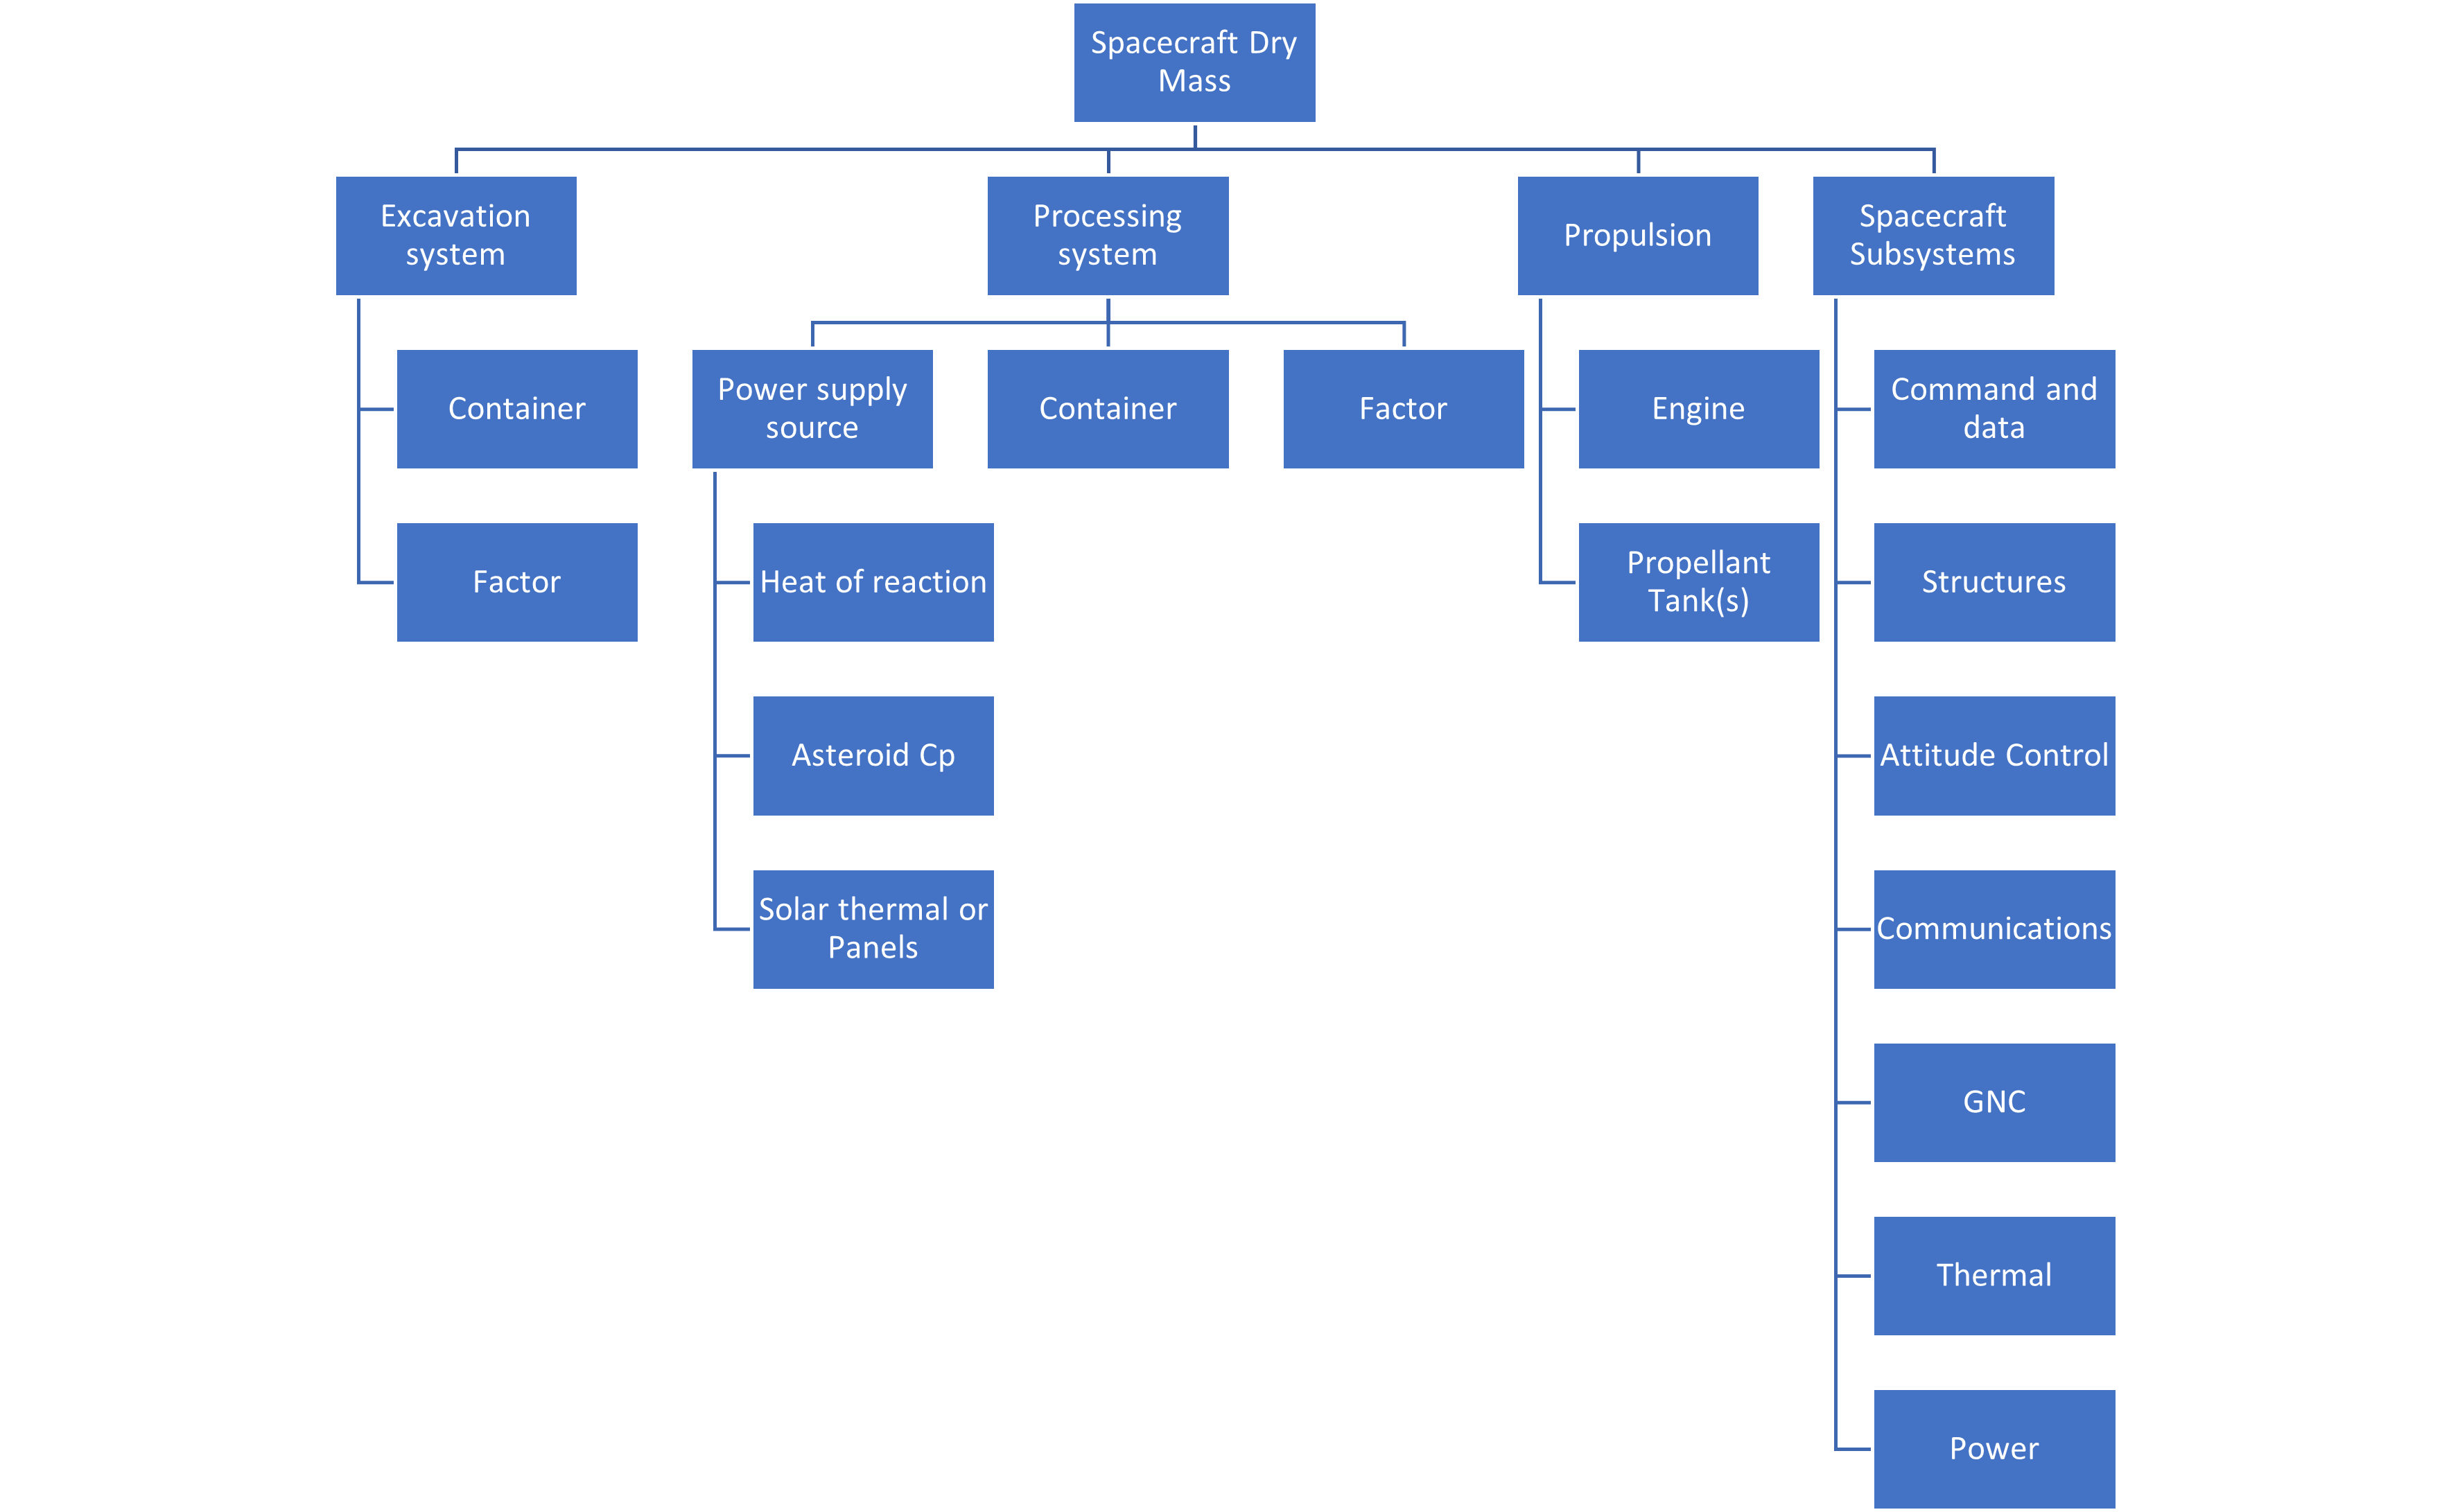
\includegraphics[width=0.9\linewidth]{mass structure.png}
    \caption{Spacecraft model structure for detemining dry mass.}
    \label{fig-model-structure}
\end{figure}


